\chapter{Simulations}
\section{Control strategies evaluation}
The previous chapters described the Grasshopper program simulating the behavior of the the room equipped with static panels, but our goal is to investigate the control strategies \footnote{The term control strategies is not interpreted as in the field of control system theory, it indicate the way to control the orientation of the panels so as reach a certain objective.} for the movement of the panels.\\
Therefore a quasi-static approach has been chosen. The idea is to simulate the behavior of the room in all reachable positions, analyze the obtained data, and finally find (backward) the corresponding optimal panels orientation.\\
The chosen parameters to be minimized, and therefore to be generated as result of the simulation are:
\begin{itemize}
\item heating consumption
\item cooling consumption
\item electricity consumption
\end{itemize}
at each of the 8760 hours of a year.
The limiting factor in this approach is the time required for a simulation.
Assuming the simulation for a single position has a duration of about 3 minutes, a limited choice of positions has to be used.\\
Another investigation option is simulation automation. The recommended way to automate the DIVA for grasshopper simulation is to use the animate function of the numeric slider [5]. This is an integrated function of Grasshopper (by right clicing in the slider).\\
The two main advantages of this method are: simplicity and automatic adaptation to the time required for the simulation.\\
An automation made by a script, how vary the panel position is instead not possible because the time required to simulate each position is different.

\section{Panel position selection}
A slider was automated to move between -90 and 90 degrees in 12 steps to control the rotation on the vertical axis. All panels move together since there is no particular benefit in combining different vertical rotations in the same fa\c{c}ade.\\
Previous researches has shown that the optimal horizontal rotation of the panels is not uniform in the entire fa\c{c}ade, especially for comfort optimization. [6]\\
The horizontal rotation affects the profoundness with which the light penetrate inside the room. Therefore three groups, of two lines of panels, were set.\\
The three chosen degrees of rotation are: $0 ^\circ$, $45 ^\circ$  and  $90 ^\circ$. This positions were called 1,2 and 3 respectively. These three numbers are assigned to identify the combination in which the simulation is made, and are used to identify the combinations in the results (see Figure~\ref{123}).\\
The total number of evaluated positions and accordingly of simulations is:
\begin{equation}
   \textbf{3} ^{ \textbf{3}} \times  \textbf{12} =  \textbf{324} 
\end{equation}
This amount of positions is a satisfactory starting point to indicate the direction in which a more precise analysis can continue.

\begin{figure}[h]
 \centering
 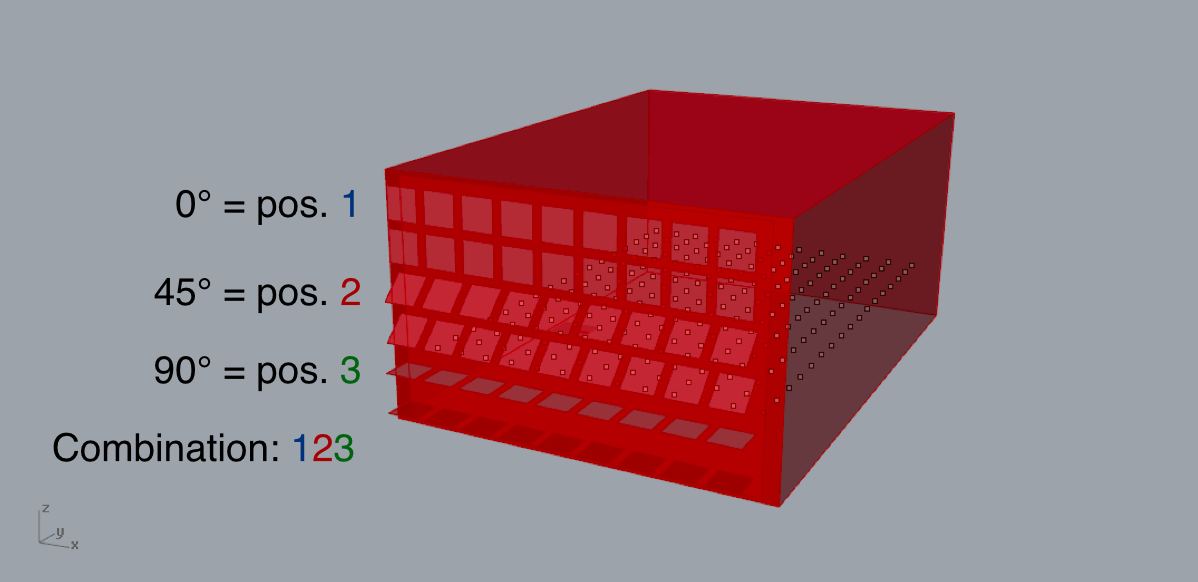
\includegraphics[width=140mm]{graphic/123.png}
 \caption{Horizontal Combinations}
 \label{123}
\end{figure}